\chapter{Pithos Design and Implementation}
\label{chp:DESIGN}

The generic state consistency model was presented in Section \ref{generic_event_update_model}. One of the key challenges that still remain was determined to be designing a root storage module specifically tailored to P2P MMVEs. The root storage model identifies in Section \ref{generic_event_update_model} includes the processes of state management and state persistency for the authoritative objects.

We've identified the main requirements of P2P MMVE state management and persistency in in Section \ref{key_challenges_cm} as: scalability,
reliability, fairness, responsiveness and security. In Chapter \ref{p2p_MMVE_state_persistency} it is argued that none of the current approaches to state persistency satisfy all identified requirements,

The focus of this thesis is, therefore exclusively on state management and persistency in P2P MMVEs. This chapter presents a design that satisfies all the identified requirements, along with implementation details and results.

Pithos, a novel hybrid multi-tiered state persistency architecture is
proposed. The novelty of Pithos lies in its support for both a responsive and a fair storage system, while also taking into account security aspects
of distributed storage. There are some storage systems that provide responsive or fair storage, but none that provide both. No storage system, designed specifically for P2P MMVEs, have taken security into account.

If Pithos is incorporated into an existing P2P MMVE consistency architecture, it will add the ability to handle both state management and state persistency. The addition of a robust state persistency mechanism, specifically designed for P2P MMVEs, will bring us one step closer to
the creation of a complete P2P MMVE architecture.
%%%%%%%%%%%%%%%%%%%%%%%%%%%%%%%%%%%%%%%%%%%%%%%%%%%%%%%%%%%%%%%%%%%%%%%

\section{Use cases}

The purpose of Pithos is to allow for efficient object storage and retrieval that satisfies all identified requirements. As is evident from root storage in the flow diagram in Figure \ref{fig_event_update_flowdiagram}, Pithos will interface directly with the VE logic, as well as receive updates from the update generator. For the purposes of this discussion, update generation is assumed to be part of game logic.

\begin{figure}[htbp]
 \centering
 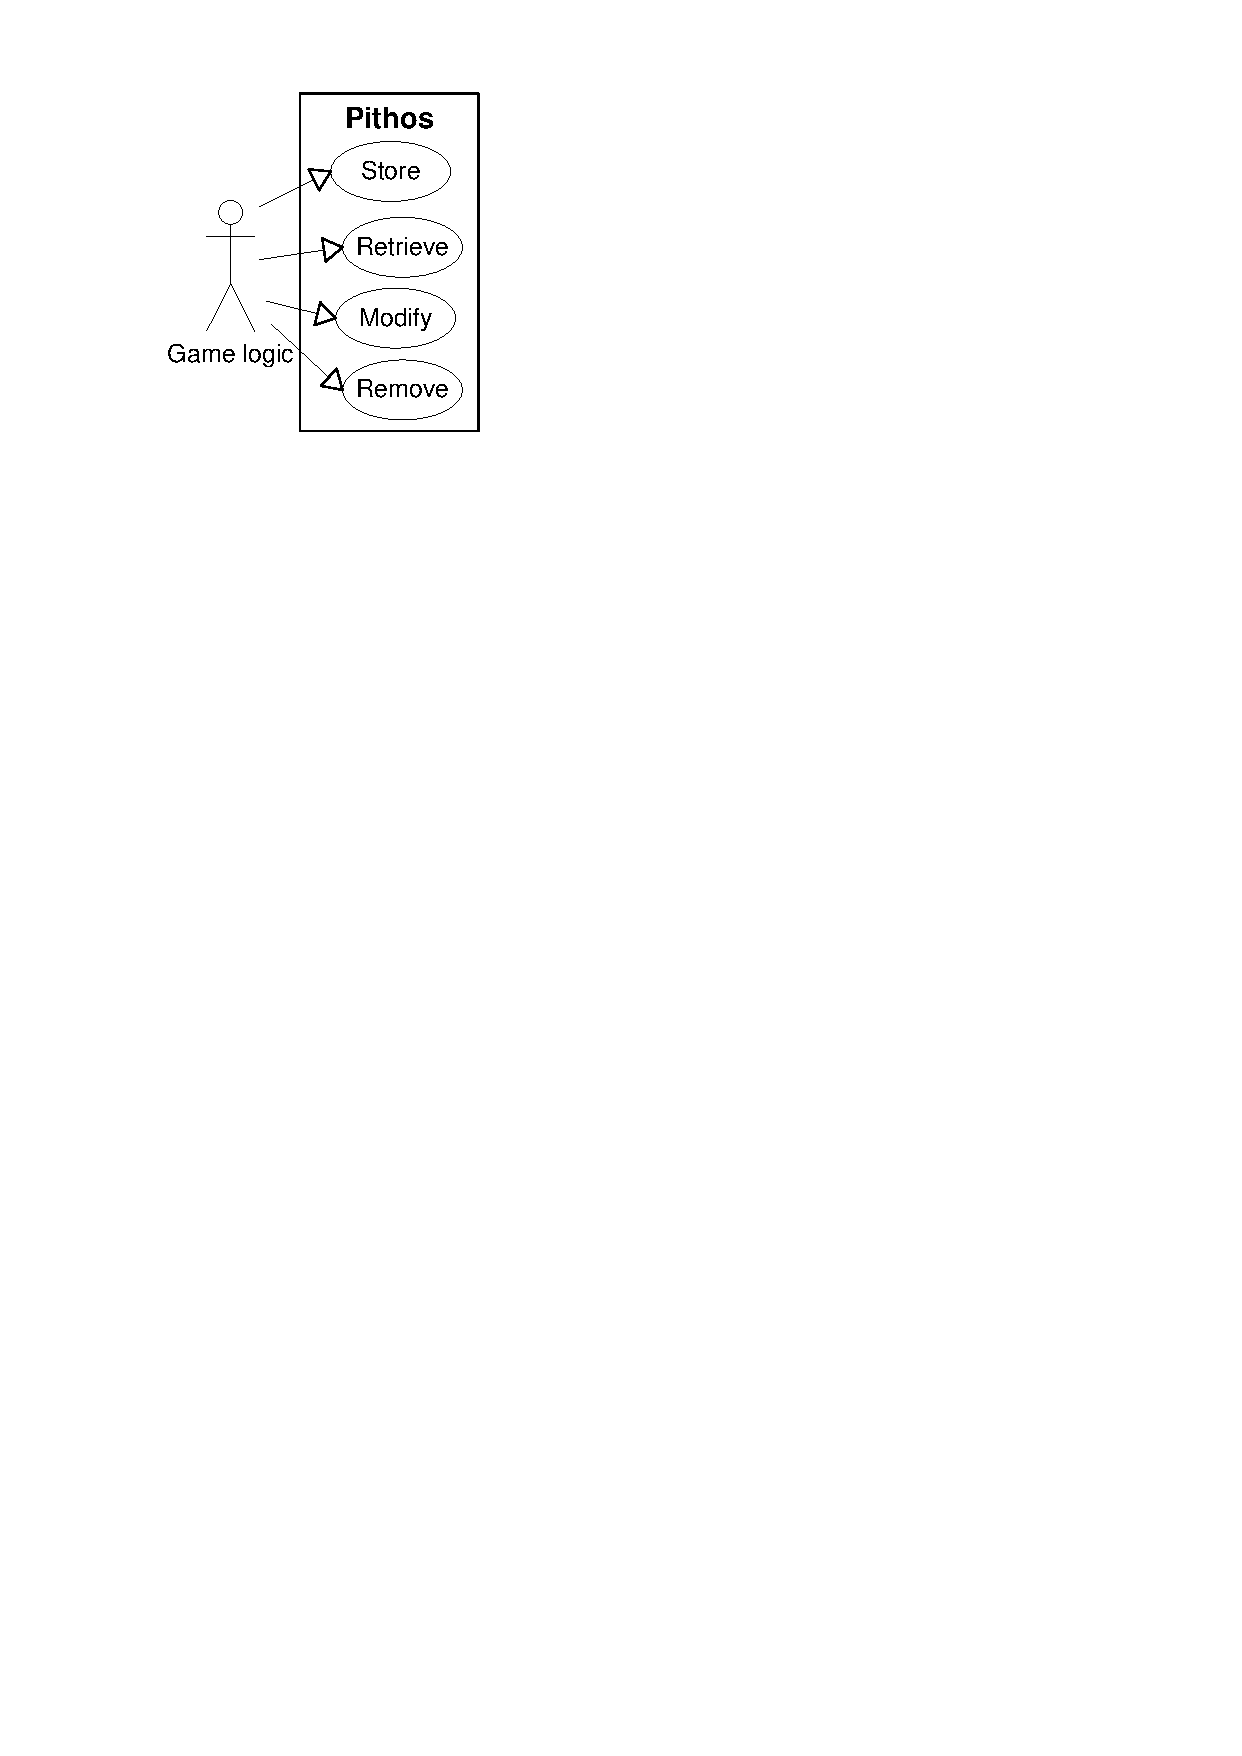
\includegraphics[clip=true, viewport=28mm 223mm 82mm 282mm, width=0.3\textwidth]{pithos_use_case}
 \caption{Use case diagram of Pithos}
 \label{fig_pithos_use_case}
\end{figure}

As shown in the use case diagram in Figure \ref{fig_pithos_use_case}, the VE logic should be able to use Pithos in four ways: store, retrieve, modify and remove. These are the use cases generally required of any storage system.

The VE logic will store data when a new object is added to the VE state. This can happen as a consequence of an event leading to the generation of a new object. An example of this is a rocket firing at a target. This event might generate a missile object to be sent towards the target.

Object retrieval will be required every time an event is received. The VE logic will retrieve the object state from memory, which is part of state management. Object states, other than the one being altered, might also be required by the logic to determine the effect an event will have, as discussed in Section \ref{event_logic_update}.

Object modification occurs every time an object update is generated. An object update, by definition, required a modification of the object state.

Object removal might also be required to save storage space, although this is not essential to the correct functioning of the storage system.

\section{Design goals}

Pithos is designed to fulfill all use case requirements as well as the requirements for P2P MMVE storage architectures as set out in Section \ref{key_challenges_cm}.

In order to fulfill the P2P MMVE storage requirements, the following design decisions were made:

The inspiration for Pithos come from two observations:
%
\begin{enumerate}
  \item One can combine multiple storage models and arrive at a model which possesses fewer disadvantages than any of the models used.
  \item Responsiveness is greatly increased in a fully distributed model, where there is no intermediate server that relays all information.
\end{enumerate}

Fully distributed architectures are, however, not scalable because the number of messages scaling by $O(N^2)$, where $N$ is the number of nodes in the network.

\section{Architecture}

\begin{figure}[htbp]
 \centering
 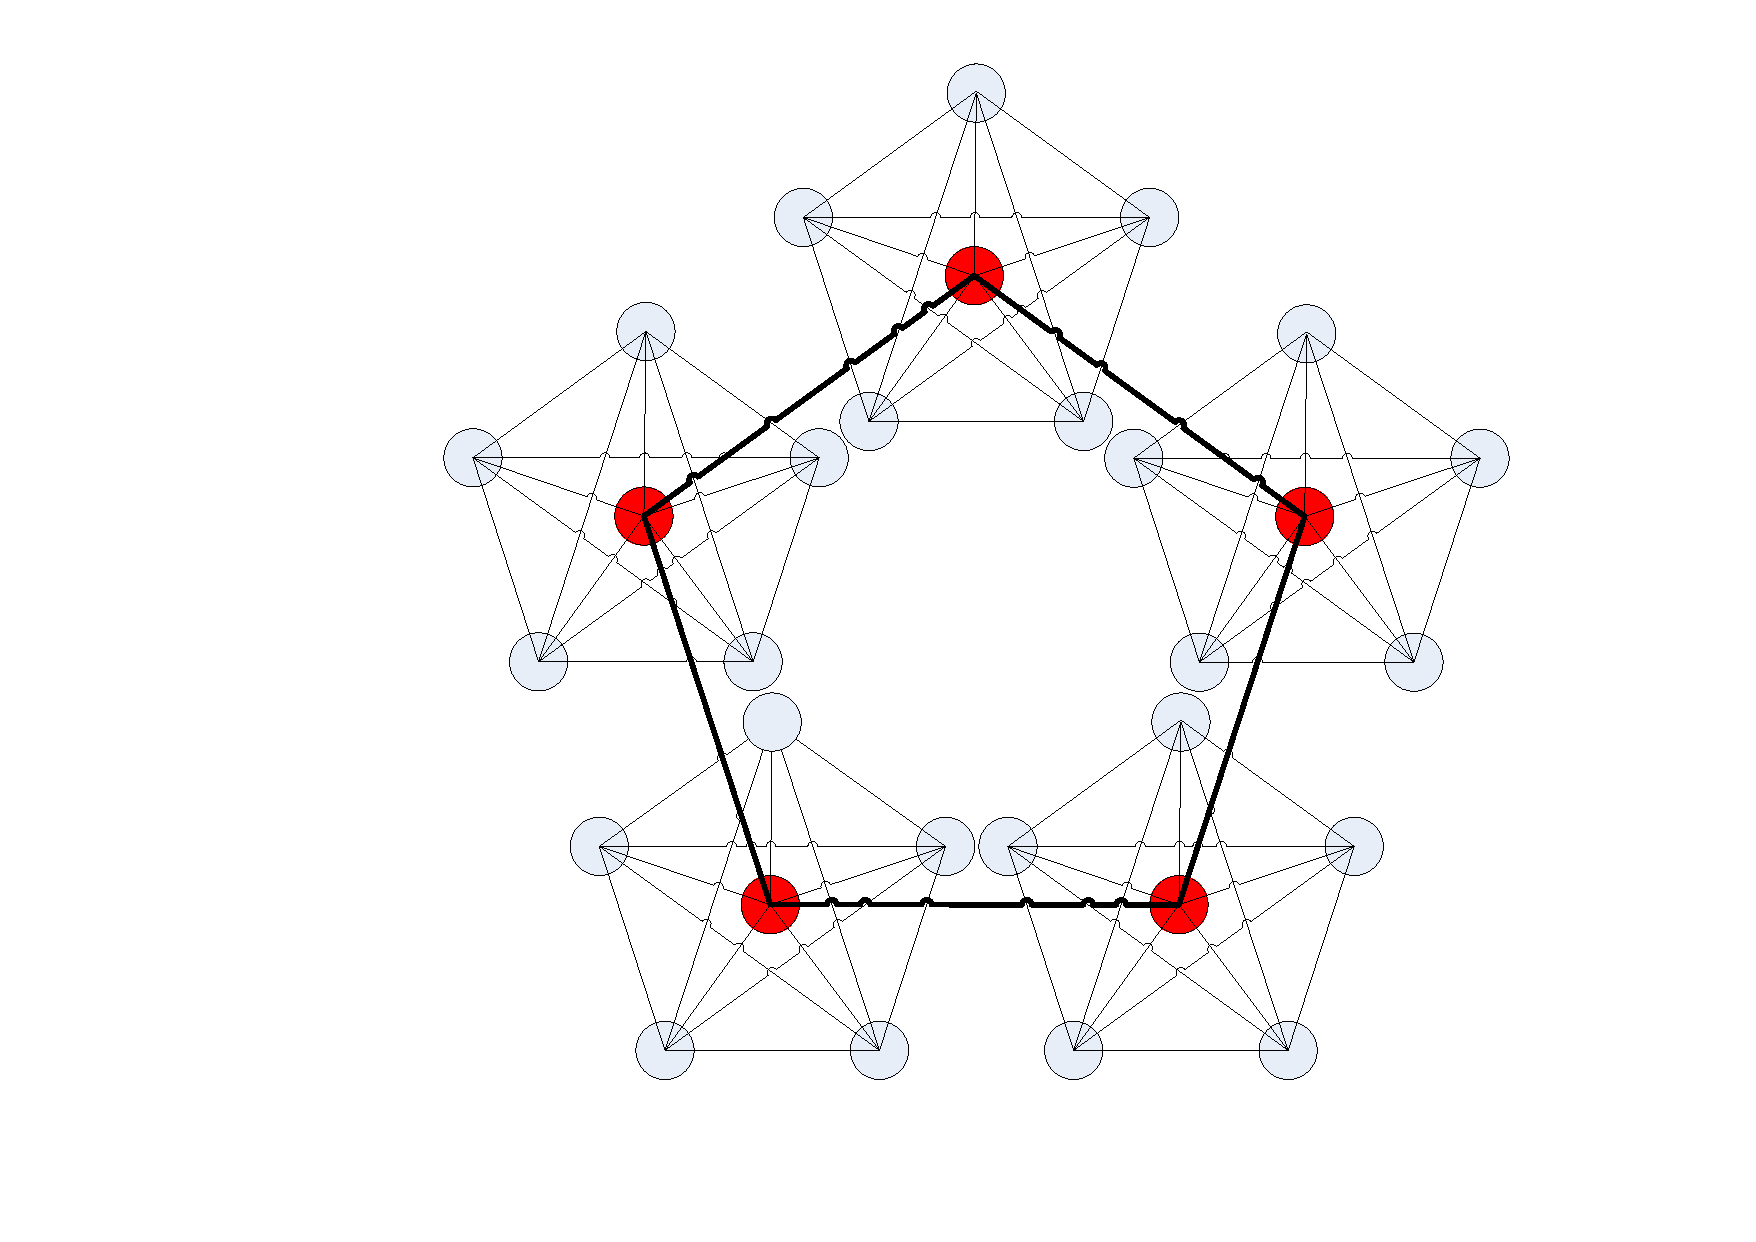
\includegraphics[clip=true, viewport=7.5cm 2.5cm 26cm 20cm, width=0.7\columnwidth]{CDHT_layout}
 \caption{Layout of the Pithos storage architecture}
 \label{fig_pithos}
\end{figure}
%
Figure \ref{fig_pithos} shows the Pithos architecture. The figure shows groups of fully connected peers (light blue and dark red), where all groups
are connected to each other in an P2P overlay through super peers (red).

Pithos groups peers to form a two tiered storage model. The first tier is a storage model at group level and the second is a storage model over all
groups. On the first tier, which is the intra-group level, a fully distributed storage system is used to allow for highly responsive read and write operations within the group. On the second tier, which is the inter-group level, a P2P overlay is used to store data between groups.

According to categorisation of \ref{storage_type_overview}, Pithos is a type of hybrid storage, that incorporates overlay storage and distance-based
storage. Responsiveness is achieved by constructing fully connected networks amongst groups of players and then storing objects that are mostly used
by the group within the group, as described in Sections \ref{grouping}, \ref{store_retrieve} and \ref{distance_based}. Reliability is achieved by
making use of replication and migration mechanisms as described in Section \ref{store_retrieve}. Security is achieved by using a certification
authority to assign node IDs and signing any storage and retrieve request with the requesting node's certificate, as described in Section
\ref{secure_ids}. Fairness is achieved by having all nodes store objects, as described in Sections \ref{store_retrieve} and \ref{distance_based}.

\subsection{Grouping}
\label{grouping}

%Speak more concretely of grouping algorithms
At the core of the architecture is the peer clustering mechanism. Two approaches are being evaluated: distributed clustering techniques (for example
affinity propagation \cite{affinity_propagation}) and dynamic regioning techniques (for example self-organising spatial publish subscribe (SOSPS)
\cite{self_organising_sps_post}).

\emph{Distributed peer clustering techniques}: make use of the flocking behaviour of players to dynamically group players into flocks or clusters
\cite{flocking}. The main idea of flocking is that players move around in groups, rather than randomly on their own. It is desirable that user
density within groups should remain constant, because a fully distributed architecture is not scalable. This means that groups should merge or split
as the user density within them change.

Affinity propagation clusters nodes using a similarity matrix to find similar nodes. The similarity matrix may contain user positions. In this case,
affinity propagation will group nodes depending on their location in a virtual world. This algorithm is ideally suited to P2P applications, since it
is a distributed clustering algorithm based on message passing.

\emph{Dynamic regioning}: divides the virtual world into regions that can be resized or further divided to maintain constant player densities across
regions. SOSPS creates dynamic regions based on a Voronoi overlay network \cite{voronoi_diagrams_survey}. Near constant user density is achieved by
increasing and decreasing the area sizes. This system is based on VON, a distributed Voronoi overlay network designed for MMVEs \cite{VON_VAST}.

\subsection{Replication}
\label{store_retrieve}

When storing objects in Pithos, replication is used to increase object availability under network churn and for security in the presence of malicious
nodes \cite{storage_and_chaching_PAST}. For every object that is stored in Pithos, $k$ object replicas are also stored. The number of replicas ($k$)
depends on the degree of network churn as well as the number of expected malicious users in the network. If the network churn is high, more replicas
are required to avoid the situation where all $k$ peers hosting an object leaves the network before any object migration can be done.

If a node leaves the network and stops to transmit ``keep alive'' messages, the migration mechanism will detect this and replicate the file on
another node. Replication exists intra- as well as inter-group and is useful in ensuring that if a nodes leaves the network, the data are not lost.
All object requests are routed to the peer with the next closest ID if the root peer leaves, because of how overly routing functions. The new
destination peers will possess the stored files, since Pithos stores overlay replicas at overlay neighbours.

Another reason to replicate game objects is to make the system more secure. If it is known that a certain percentage of users are malicious, it is
advantages to have more replicas than malicious users. This will allow for a secure system where object hashes can be compared to determine which
nodes are malicious and what version of an object is accurate.

\subsection{Distance-based storage}
\label{distance_based}

For Pithos to succeed as an MMVE storage architecture, intra-group data requests should be preferred to inter-group data requests. This requirement,
combined with the fact that the grouping algorithm geographically groups players in the virtual world, lends Pithos to a storage system based on
distance-based storage. Similar to interest management, the assumption is that players have a limited area of interest and require interaction with a
limited number of objects within range.

Therefore, distance-based storage is implemented on a group level rather than an individual level. This means that objects are stored on the nearest
group of players, rather than the nearest user. It is assumed that such an approach will alleviate the security and reliability challenges present in
distance-based storage \cite{gilmore_p2p_mmog_state_persistency}.

With group-based distance-based storage, it is assumed that because peers now store objects closest to the group, the objects that they are
interested in will most likely be stored within their own group. Therefore, most data requests should be intra-group requests. The overlay storage
component ensures that nodes that require data, which are not stored within their group, are still able to access requested data.

\subsection{Secure storage and node ID assignments}
\label{secure_ids}

In order to design a secure distributed storage system, one requirement for the P2P overlay is that nodes should not be able to select their own IDs
or it will not be possible to secure the system against attack. Node IDs should rather be assigned securely by some certification authority
\cite{secure_overlay_routing}.

To meet this requirement, Pithos implements its own certification authority to assign node IDs securely and promote security in the P2P overlay. A
certification server exists that handle ID requests from nodes. The server assigns IDs to nodes and provides the node with a signed certificate that
it may use to store data.

Whenever an object is stored or updated in the storage network, nodes have to sign the object to enable the tracking of object changes throughout the
life of the object. This system is very different from classic distributed file storage designs that advocate anonymity in storage. The fact that all
changes can be tracked to a specific node will simplify the task of eliminating user cheating.

\section{Oversim}

Pithos has been implemented in Oversim \cite{OverSim_2007}, a P2P simulation environment based in Omnet++, which allows for the measurement of identified requirements. Furthermore, it allows for the comparison of the current model with other state persistency models.

Oversim is a peer-to-peer and overlay network framework for the Omnet++ simulator. Oversim allows for the simulation of many well known structured or unstructured overlay protocols. It also allows for the development of applications that can use the already implemented overlays in a well defined architecture.

    \subsection{Motivation}

To allow for greater control of the environment, as well as greater scale, it was decided to implement the first version of Pithos as a large scale network simulation. A simulation allows for careful selection of the environment parameters and tight control of the parameter values. This in turns allows one to keep all but one parameters constant and evaluate the effect of a design decision on the system for varying values of the free parameter.

The underlying Omnet++ simulation environment is a powerful network simulator in its own right. It allows for robust message and module definitions and contains many tools to assist with simulation measurement and monitoring.

Simulation also allows for greater scalability and simulating on a network with global Internet characteristics. Greater scalability is achieved, because thousands of nodes can easily be created, where all the nodes have global scale latency characteristics.

Implementing a large scale network application in the real-world would require thousands of computers spread across the globe. Such an environment will contain many variables out of the designer's control. Issues such as router congestion for example varies from day to day, which will produce varying latency results.

Because of these reasons, it was decided to first implement Pithos in simulation. This allows for the perfection of the design, under laboratory conditions, before the real world implementation is completed.

Pithos is intended for future real world implementation, however, so all modules created were written in such a manner to allow for easy porting. No tasks that are performed in Pithos make use of any simulation ``short cuts'', such as accessing the global peer list. Only statistics gathering modules are allowed to make use of these simulation features.


    \subsection{Architecture}

        \subsubsection{Layers}
        
\begin{figure}[htbp]
 \centering
 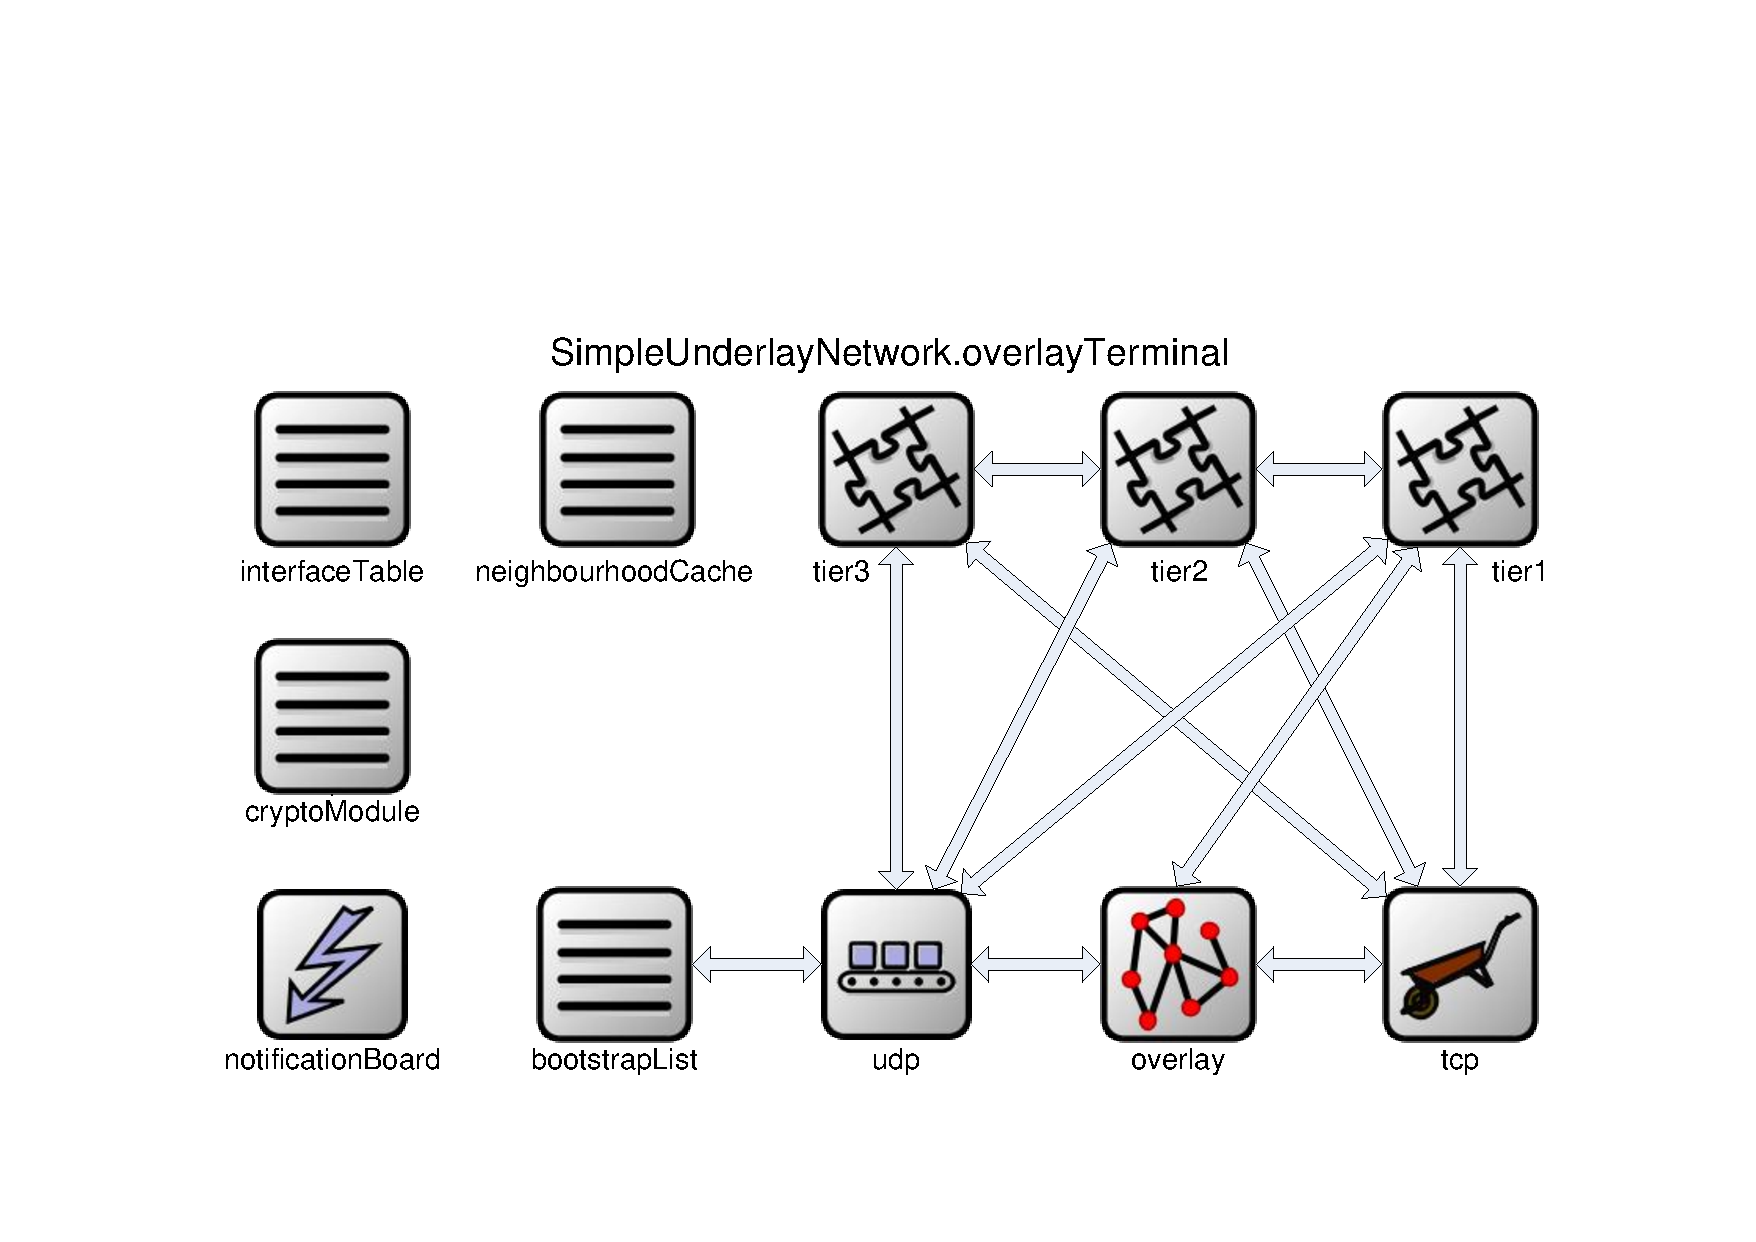
\includegraphics[clip=true, viewport=33mm 27mm 262mm 197mm, width=\columnwidth]{Oversim_architecture}
 \caption{The default}
 \label{fig_oversim_architecture}
\end{figure}

\begin{figure}[htbp]
 \centering
 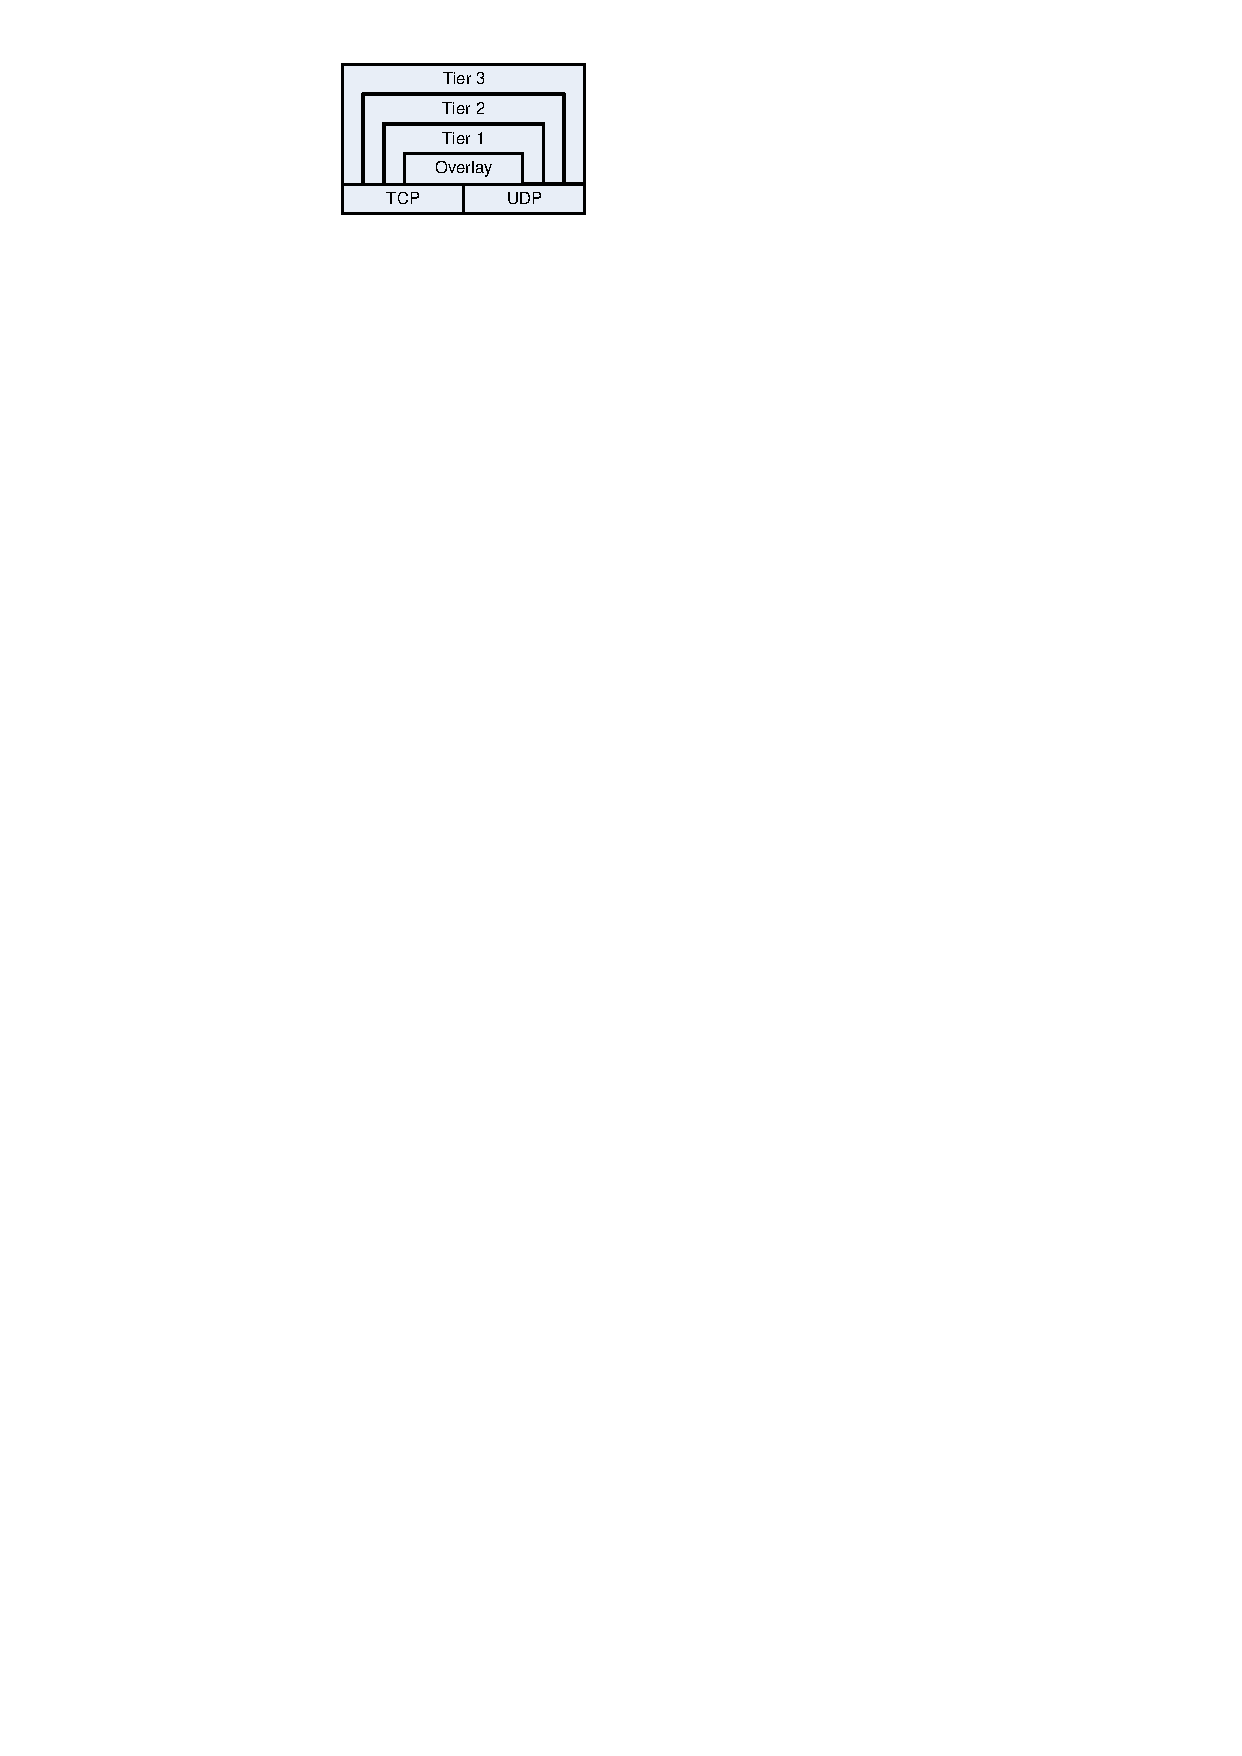
\includegraphics[clip=true, viewport=57mm 260mm 100mm 287mm, width=0.5\columnwidth]{Oversim_layers}
 \caption{Oversim architecture layers}
 \label{fig_oversim_layers}
\end{figure}

%Also show the Oversim picture

Oversim is a layered architecture, as shown in Figure \ref{fig_oversim_layers}. The Oversim architecture contains the layers: TCP, UDP, Overlay, Tier 1, Tier 2 and Tier 3.

The transport control protocol (TCP) and user datagram protocol (UDP) are both transport level protocols, according to the OSI protocol stack specification. These two layers are the lowest communications layers in Oversim and allows message passing to other nodes.

The overlay layer is where the P2P overlay is housed. This can be any of the well known structured or unstructured overlays, such as Pastry, Chord or Gia. The three tiers above the overlay layer are the application level layers and is where application that use an overlay may be implemented. Three application layers are allowed.

Tier 1 can communicate with the Tier 2, overlay, TCP and UDP layers. Tier 2 can communicate with the Tier 1, Tier 3, TCP and UDP layers. Tier 3 can communicate with the Tier 2, TCP and UDP layers. Internal communications are usually between tiers and TCP and UDP communication occurs when a layer wishes to send a message to the same layer on a different node.

        \subsubsection{Churn generators}

Oversim also contains the concept of a churn generator. Churn generators model users joining and leaving the network. There are three types of churn generators: ``no churn'', ``lifetime churn'' and ``Pareto churn''. The ``no churn'' churn generator creates nodes every specified number of seconds until a specified number of nodes are reached and does nothing further. This generator can be used to test simple networks, where churn is not an issue, or for initial testing of the first prototype.

Lifetime churn creates nodes with specified average lifetimes, sampled from an exponential distribution. This is a distribution regularly used to model lifetimes in reliability engineering. Pareto churn samples node lifetimes from a Pareto distribution, instead of an exponential distribution. This churn generator type requires mean node lifetime as well as mean node dead time to be specified.

Multiple churn generators can exist in an Oversim simulation. Each churn generator can create a unique terminal type. A terminal type is determined by the protocols executing on every layer of the Oversim architecture.

    \subsection{Generic consistency extension}

%Show the generic consistency architecture in Oversim

To allow Oversim to simulate a complete consistency architecture, the Oversim framework itself was extended. The three tiers were replaced with all the elements identified in the generic consistency model in Section \ref{generic_event_update_model}. Figure \ref{} shows the extended Oversim framework containing the following layers:
\begin{itemize}
    \item Agent
    \item Event layer IM
    \item Event dissemination
    \item Event ordering
    \item Game logic
    \item Root object updater
    \item Root object store
    \item Update layer IM
    \item Update dissemination
    \item Object merger
    \item Local object updater
    \item Local object store
    \item Display updater
    \item Overlay Storage
\end{itemize}

Every new layer can communicate with the layer above and below it, and can also communicate with its version on another node using UDP or TCP. This allows for the consistency model to be distributed amongst any number of nodes. A module can either send its information to the layer below it within the same node, or it can send it to the layer below it on another node.

Every module can contain a collection of sub-modules which implements the layer itself. It the layer is not implemented, a dummy layer may be specified. The Pithos implementation is located within the root object store module. An application that provides Pithos with test inputs called ``PithosTestApp'' is situated within the root object updater layer. Pithos also makes use of overlay storage, which is implemented in the overlay storage module. Overlay storage requires a P2P overlay for routing purposes, which is why it is connected to the overlay layer.

\section{Pithos nodes and modules}

\begin{figure}[htbp]
 \centering
 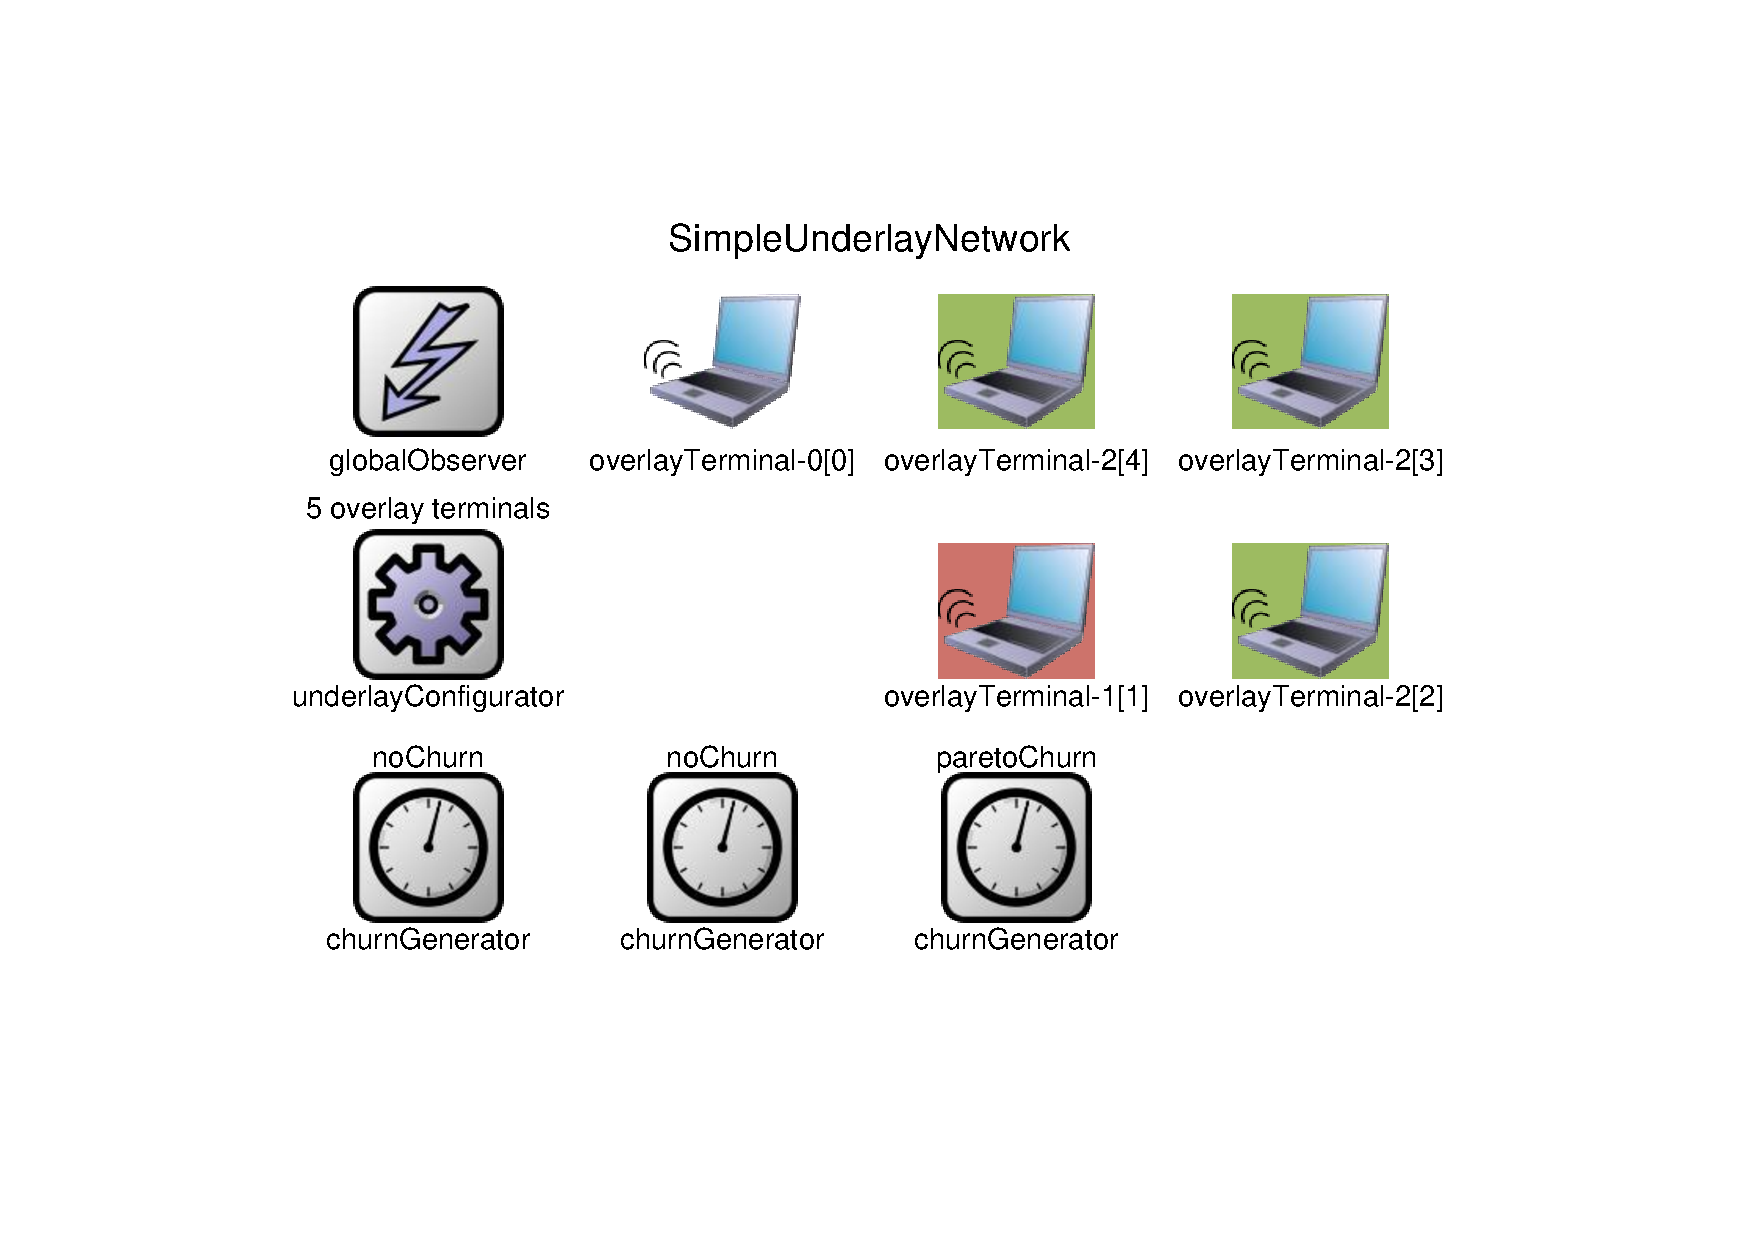
\includegraphics[clip=true, viewport=49mm 48mm 245mm 173mm, width=0.5\columnwidth]{Oversim_terminals}
 \caption{The Oversim simple underlay network with the three Pithos terminal types}
 \label{fig_oversim_terminals}
\end{figure}

Three types of Pithos nodes exist: super peers, peers and a directory server. The single directory server is a normal three-tiered Oversim node, which places joining peers into groups represented by super peers, as explained in Section \ref{network_join_iplementation}.

Super peers represent and manage groups. This includes ensuring group consistency, which is to say, ensuring that all nodes perceive the same peers as being part of their group. Super peers also inform joining peers of objects available in a group.

Peers in Pithos contain peer logic, communicator, group storage, DHT storage and group ledger modules.

In the Pithos implementation, the only difference between a super peer and a peer is that a super peer node, in addition to all peer modules, also contain super peer logic and a super peer group ledger.

\begin{figure}[htbp]
 \centering
 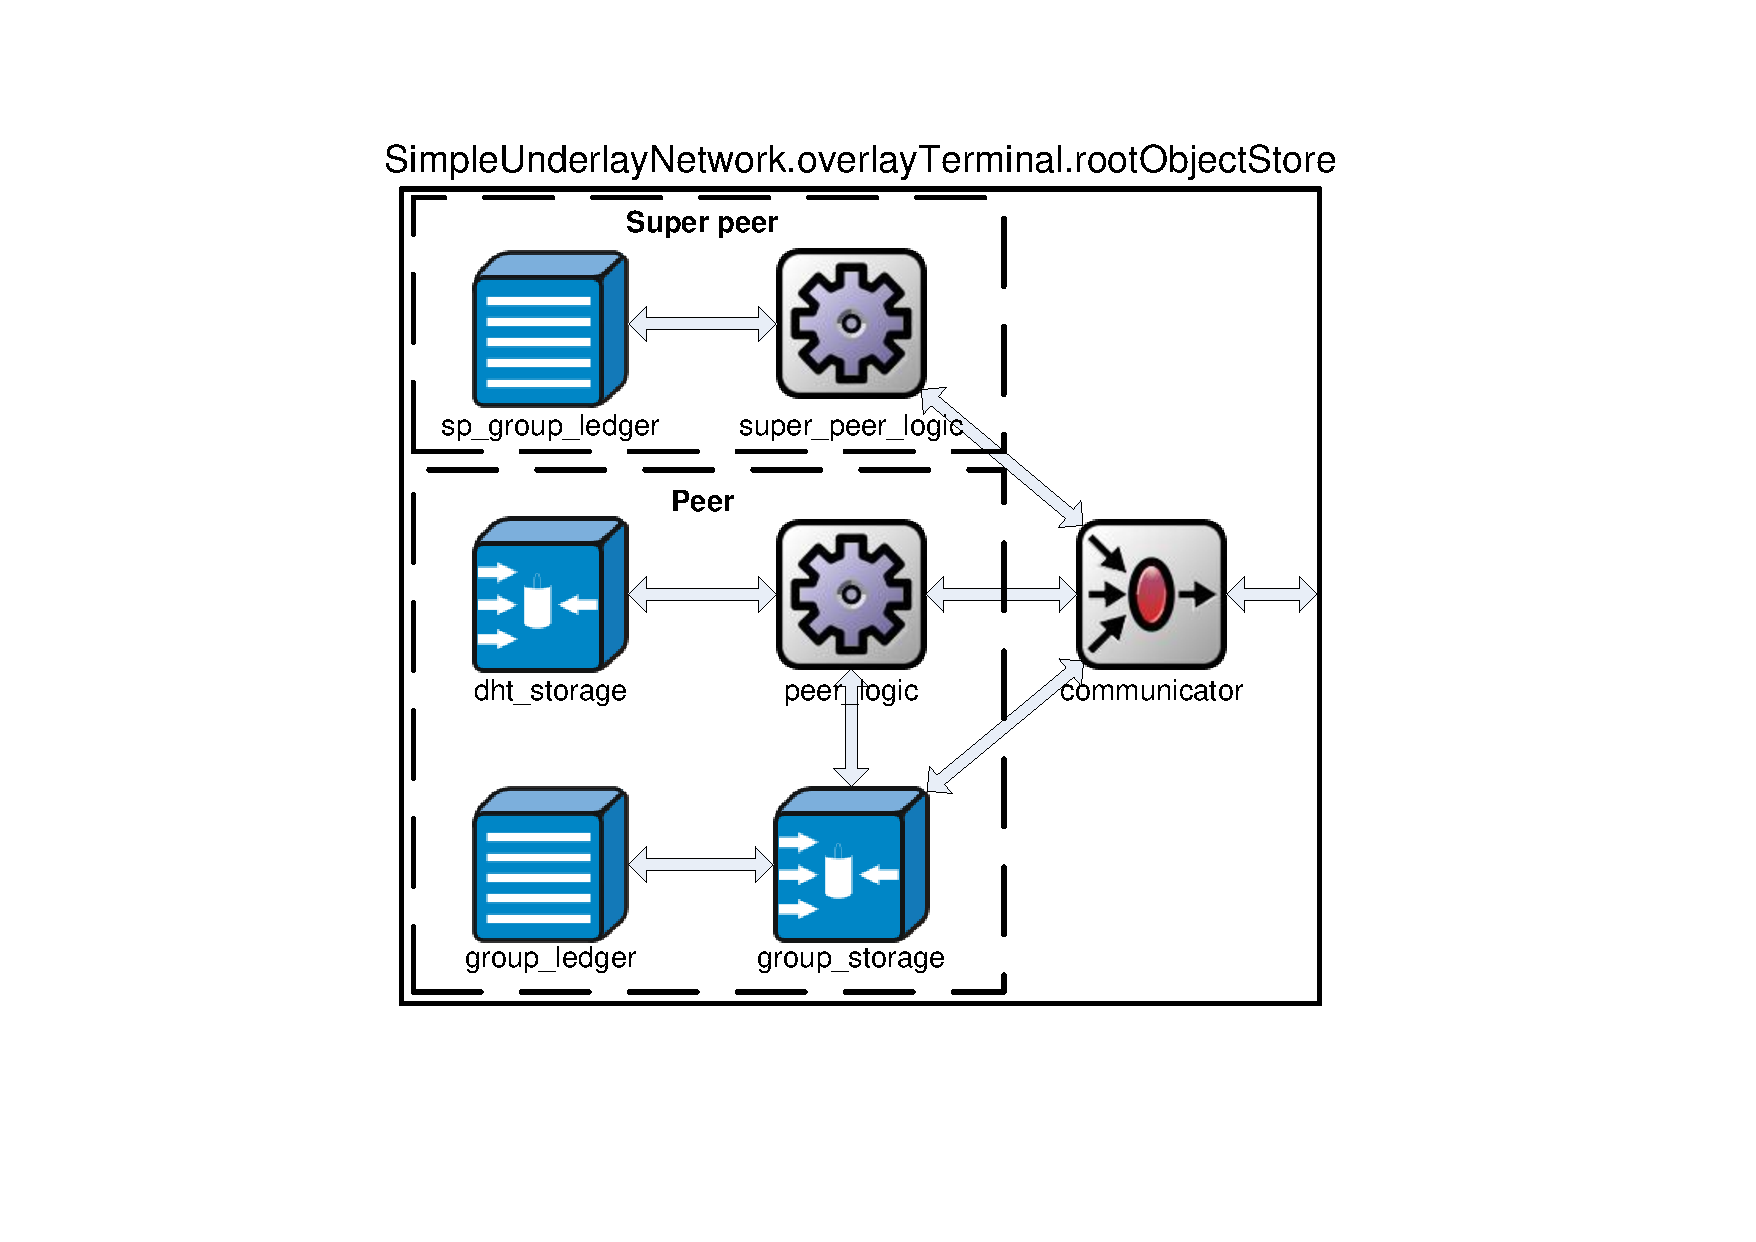
\includegraphics[clip=true, viewport=64mm 39mm 227mm 186mm, width=0.5\columnwidth]{Oversim_root_object_store}
 \caption{Pithos super peer and peer modules in Oversim}
 \label{fig_oversim_root_object_store}
\end{figure}

\section{DHT modules}
%Generic architecture required extension

\section{PithosTestApp modules}

\section{Key mechanisms}
    \subsection{Joining the network}
    \label{network_join_iplementation}
    All super peers advertise their locations with the directory server. When a

    \subsection{Grouping}

    \subsection{Storing data}

    \subsection{Retrieving data}

    \subsection{Modifying data}

    \subsection{Group migration}

\section{Designing for network churn}

    \subsection{Repair mechanisms}

    \subsection{Group consistency}
    %Check how this increases with increased network sizes and varying levels of network churn.

\section{Bandwidth requirements (overhead)}
    %Mention something about low bandwidth links and how that influences timeout and what extra mechanisms were required.
    %Check how this increases with increased network sizes and varying levels of network churn.
